\chapter{\ifproject%
\ifenglish Experimentation and Results\else การทดลองและผลลัพธ์\fi
\else%
\ifenglish System Evaluation\else การประเมินระบบ\fi
\fi}

\quad \quad ในบทนี้จะทดสอบเกี่ยวกับการทำงานในฟังก์ชันหลักของแพลตฟอร์มว่าสามารถทำงานได้
หรือไม่ โดยมีการทดสอบการทำงานต่าง ๆ ดังนี้

\section{การทดสอบโดยการการยืนยันตัวตนผ่าน google}
\quad \quad การทดสอบโดยการการยืนยันตัวตนผ่าน google จะเรียกใช้ Firebase Authentication เข้ามาช่วยในการจัดการ
โดยการทดลองจะทำการเข้าสู่ระบบยืนยันตัวตนโดยผ่านบัญชี google ผลลัพธ์คือสามารถเข้าสู่ระบบได้สำเหร็จและสามารถดึงข้อมูลส่วนตัวมาได้
ดังรูป 4.1 
    \begin{figure}
    \begin{center}
      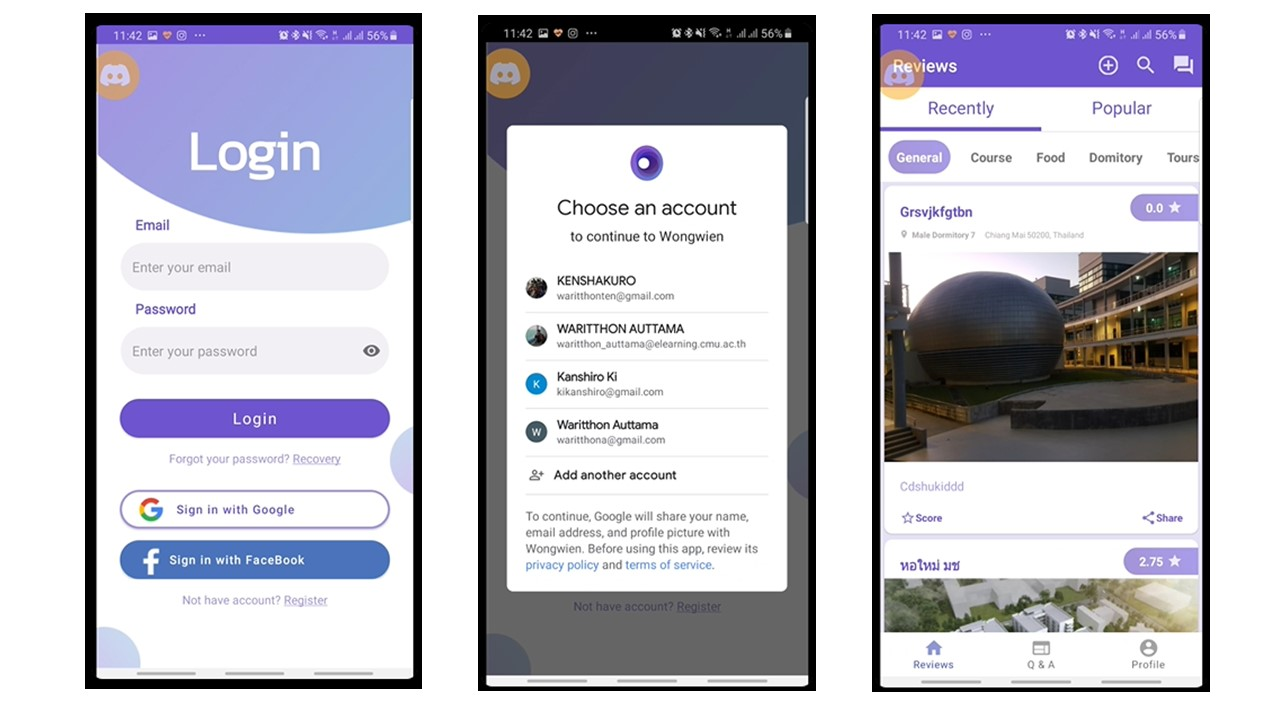
\includegraphics[width=1\textwidth]{./image/testing/Slide1.JPG}
    \end{center}
    \caption[การทดสอบโดยการการยืนยันตัวตนผ่าน google]{การทดสอบโดยการการยืนยันตัวตนผ่าน google}
    \end{figure}

\section{การทดสอบโดยการการยืนยันตัวตนผ่าน facebook}
\quad \quad  การทดสอบโดยการการยืนยันตัวตนผ่านเฟสบุ๊กโดยใช้ Facebook api เข้ามาใช้ในเขียนเชื่อมต่อ และใช้Firebase Authentication 
เข้ามาช่วยจัดการระบบหลังบ้าน (Back-end) โดยการทดลองจะยืนยันตัวตนผ่านเฟสบุ๊ก ผลลัพธ์คือสามารถเข้าสู่ระบบโดยโดยใช้บัญชีเฟสบุ๊คได้ และสามารถดึง
ข้อมูลผู้ใช้มาได้บางส่วน ดังรูป 4.2

    \begin{figure}
    \begin{center}
      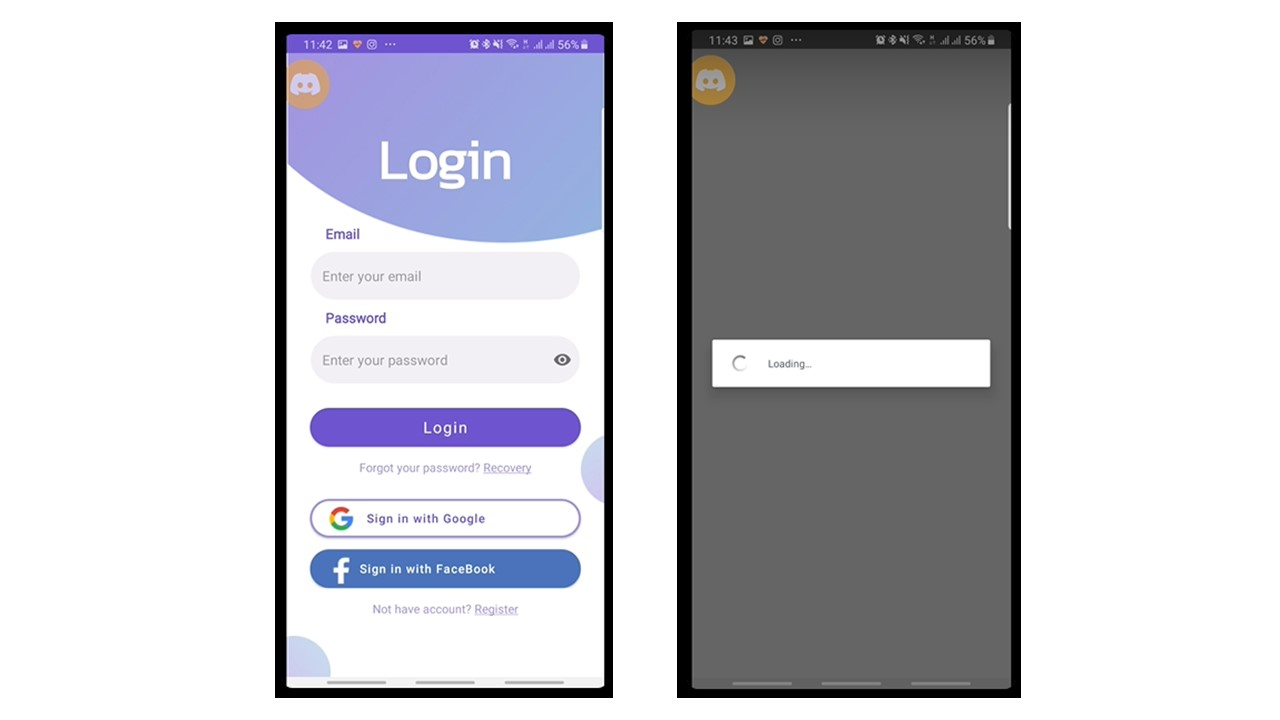
\includegraphics[width=1\textwidth]{./image/testing/Slide2.JPG}
    \end{center}
    \caption[การทดสอบโดยการการยืนยันตัวตนผ่าน facebook]{การทดสอบโดยการการยืนยันตัวตนผ่าน facebook}
    \end{figure}


\section{การทดสอบการใช้กูเกิลแผนที่ (Google map)}
\quad \quad การทดสอบเข้าใช้งาน google map โดยการจำลองการเพิ่มรีวิวได้มีการแท็กสถาที่ ซึ่งจะมาเรียกใช้งานตัว google map api เพื่อหาตำเเหน่งสถานที่ปัจจุบัน
ผลลัพธ์การทดลองคือ สามารถเข้าถึงตำแหน่งของเราปัจจุบันและสามารถดึงข้อมูลพิกัดตำแหน่งของเราได้ดังรูป 4.3
\begin{figure}
    \begin{center}
      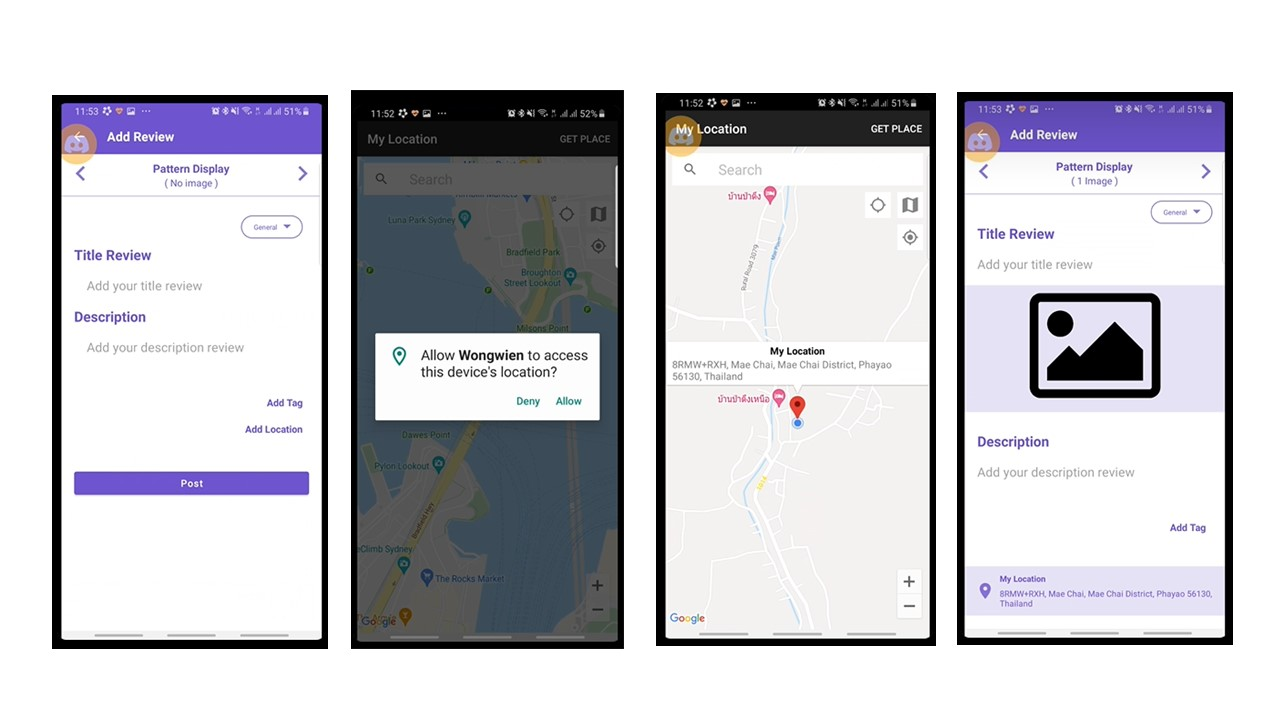
\includegraphics[width=1\textwidth]{./image/testing/Slide3.JPG}
    \end{center}
    \caption[การทดสอบการใช้กูเกิลแผนที่]{การทดสอบการใช้กูเกิลแผนที่ (Google map)}
    \end{figure}

\section{การทดสอบการเพิ่มรีวิว}
\quad \quad  การทดสอบเพิ่มการรีวิวโดยให้ทำการสร้างโฟสรีวิวขึ้นมา มีการตั้งหัวเรื่องรีวิว แนบรูป บรรยาย ติดแท็กต่างๆและมีการเเท็กสถานที่
ผลลัพธ์คือสามารถเพิ่มการรีวิวได้สำเหร็จและครบถ้วน ดังรูป 4.4
\begin{figure}
    \begin{center}
      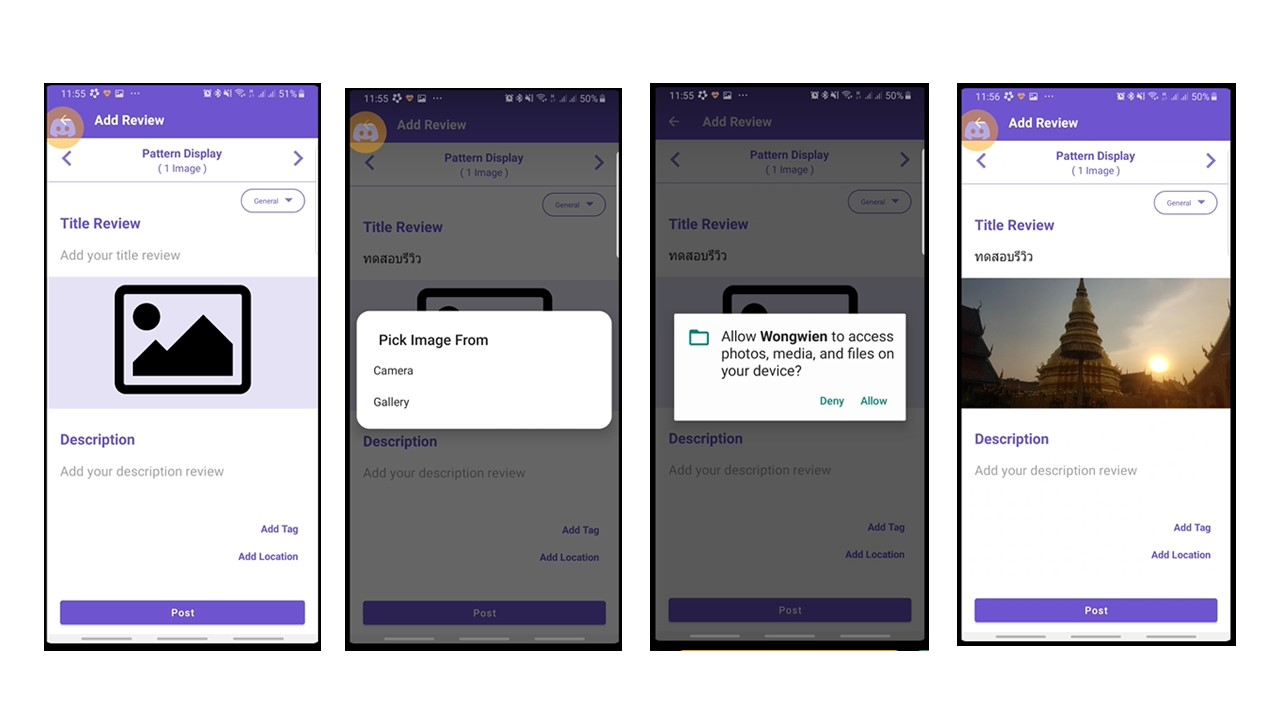
\includegraphics[width=1\textwidth]{./image/testing/Slide4.JPG}
    \end{center}
    \end{figure}

    \begin{figure}
        \begin{center}
          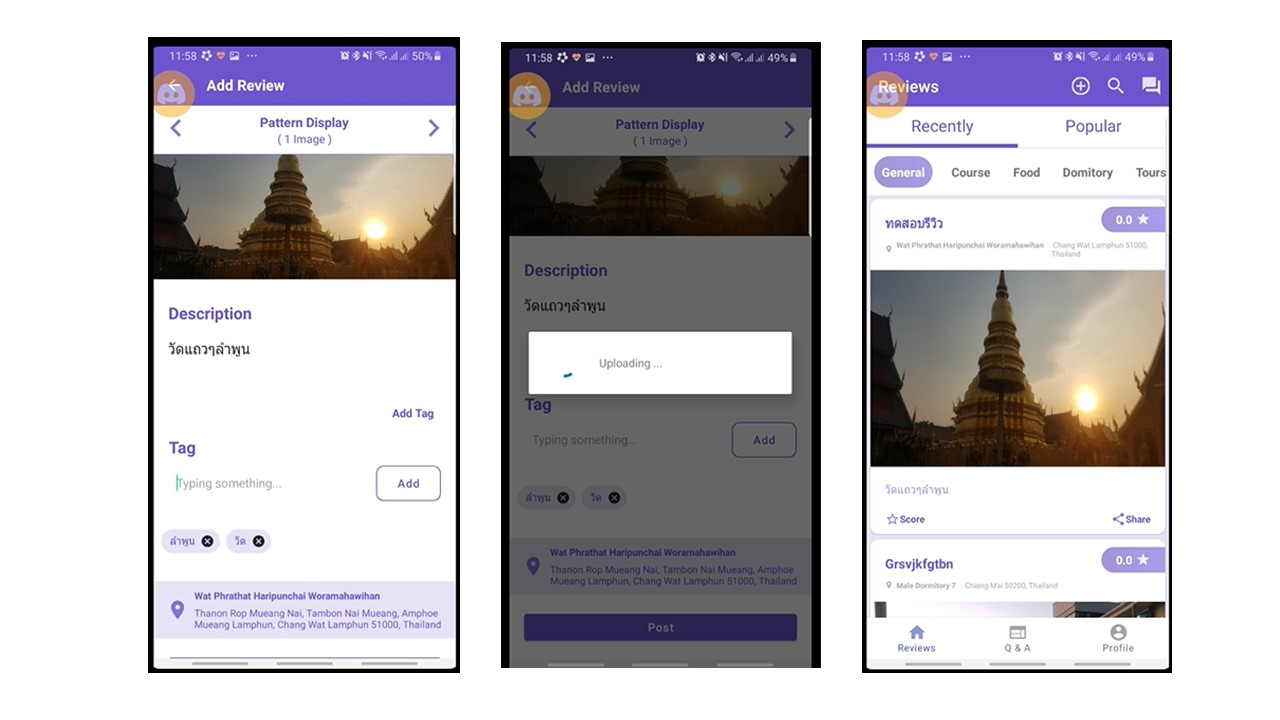
\includegraphics[width=1\textwidth]{./image/testing/Slide5.JPG}
        \end{center}
        \caption[การทดสอบการเพิ่มรีวิว]{การทดสอบการเพิ่มรีวิว}
        \end{figure}

\section{การทดสอบการให้คะแนนรีวิว}
\quad \quad การทดสอบการให้คะแนนรีวิว โดยให้ทำการให้คะแนนดาวรีวิว การคำนวนคะแนนรีวิวมาจากการเฉลี่ยของคนที่ให้ตะแนนรีวิว
ผลการทดสอบคือสามารถให้คะแนนดาวรีวิวได้สำเหร็จและคำนวนได้ถูกต้องดังรูป 4.5
\begin{figure}
    \begin{center}
      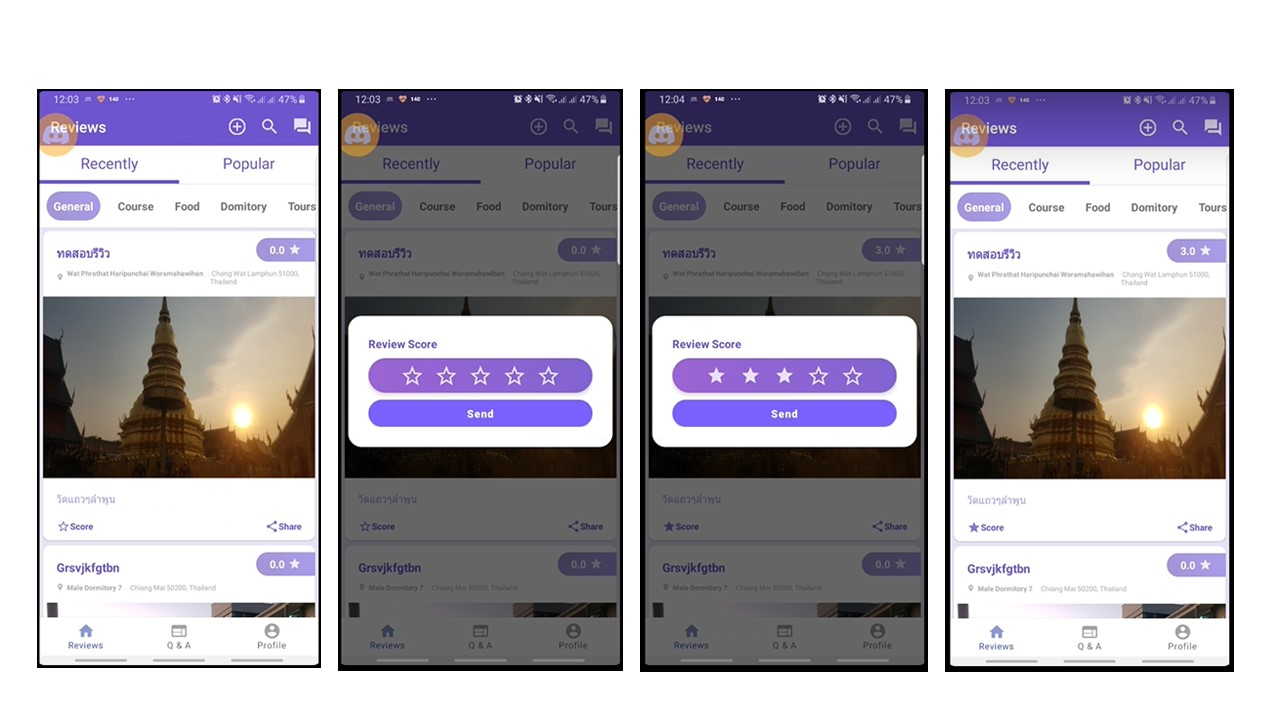
\includegraphics[width=1\textwidth]{./image/testing/Slide6.JPG}
    \end{center}
    \caption[การทดสอบการให้คะแนนรีวิว]{การทดสอบการให้คะแนนรีวิว}
    \end{figure}

\section{การทดสอบการให้คอมเม้น}
\quad \quad การทดสอบการให้คอมเม้น คือจะให้เข้าไปคอมเม้นในส่วนของรีวิวโดยเลือกรีวิวมาแล้วกดเข้าไปดุรายละเอียดของรีวิวจากนั้นก็
สามารถคอมเม้นรีวิวนั้นๆ ผลลัพธ์คือสามารถคอมเม้นได้สำเหร็จระบบก็จะแสดงคอมเม้นล่าสุดที่เราพึ่งคอมเม้นไป ดังรูป 4.6 

\begin{figure}
    \begin{center}
      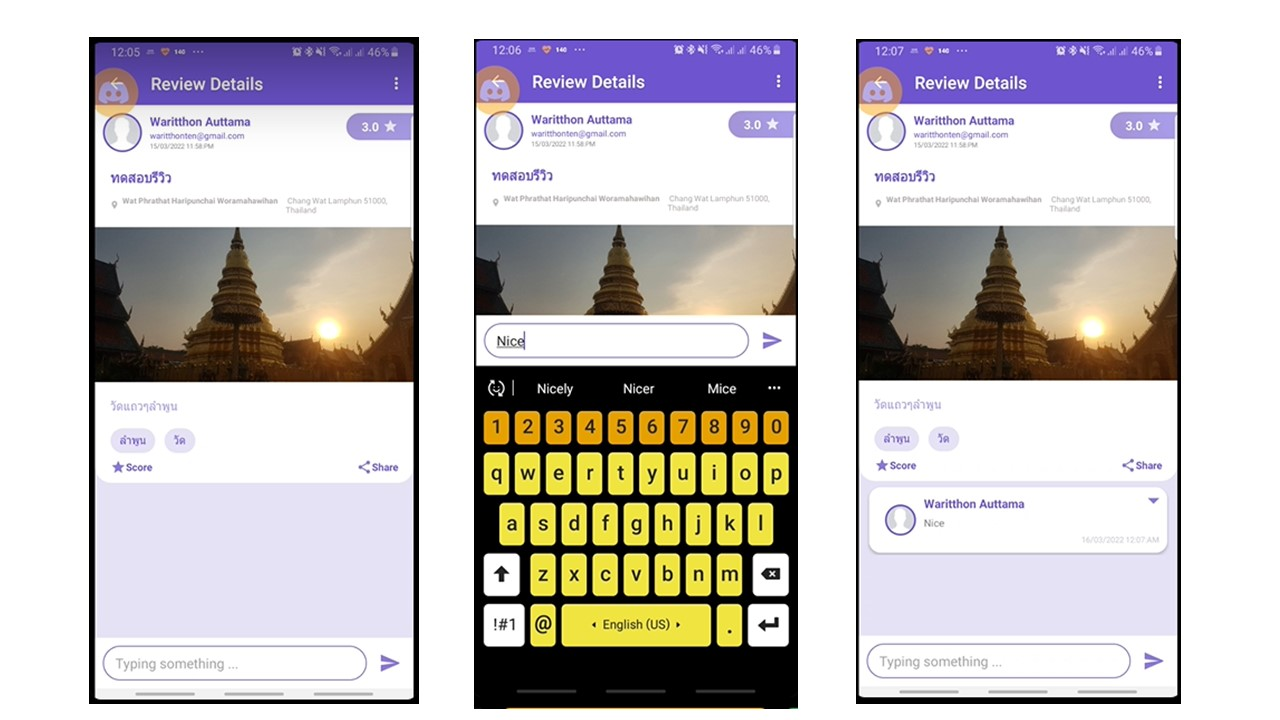
\includegraphics[width=1\textwidth]{./image/testing/Slide7.JPG}
    \end{center}
    \caption[การทดสอบการให้คอมเม้น]{การทดสอบการให้คอมเม้น}
    \end{figure}

\section{การทดสอบการแก้ไขคอมเม้น}
\quad \quad การทดสอบการแก้ไขคอมเม้น คือจะให้เข้าไปแก้ไขคอมเม้นที่เราได้คอมเม้นไปจากการทดลองก่อนหน้านี้ โดยการแก้ไขคือให้กดคอมเม้นที่เราคอมเม้นไปค้างไว้สักพักจะปรากฎเมนูแก้ไขขึ้นมา
ให้เราทำการพิมแก้ไขคอมเม้นรีวิว จกานั้นกดปุ่ม update ผลลัพธ์คือสามารถแก้ไขคอมเม้นได้สำเหร็จ ระบบก็จะแสดงคอมเม้นล่าสุดที่เราพึ่งแก้ไขคอมเม้นไป ดังรูป 4.7 

\begin{figure}
    \begin{center}
      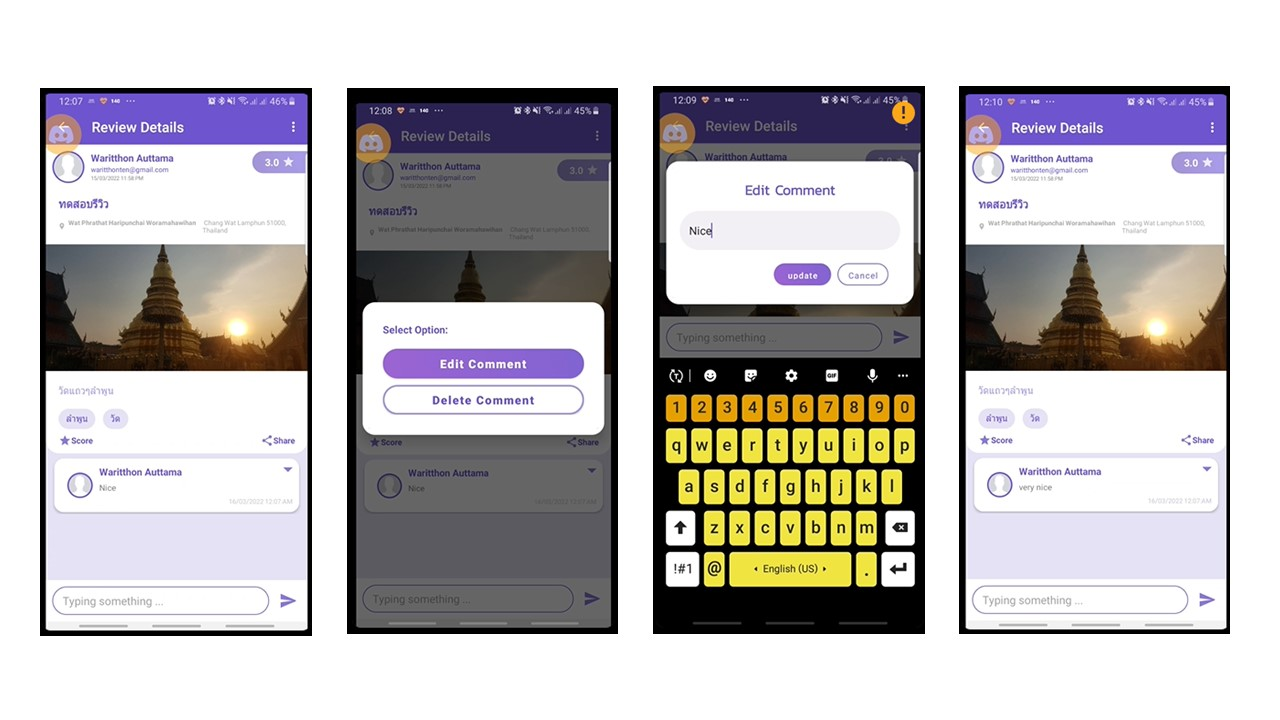
\includegraphics[width=1\textwidth]{./image/testing/Slide8.JPG}
    \end{center}
    \caption[การทดสอบการแก้ไขคอมเม้น]{การทดสอบการแก้ไขคอมเม้น}
    \end{figure}
    
\section{การทดสอบการเพิ่มกระทู้}
\quad \quad การทดสอบการเพิ่มกระทู้ คือจะให้เปิดหน้ากระทู้จากนั้นกดปุ่ม + เพื่อเพิ่มการตั้งกระทู้ เมื่อตั้งกระทู้แล้วกดปุ่มโฟส 
ผลลัพธ์คือสามารถเพิ่มกระทู้ได้สำเหร็จ ระบบจะแสดงกระทู้ล่าสุดที่เราพึ่งโฟสไป  ดังรูป 4.8

\begin{figure}
    \begin{center}
      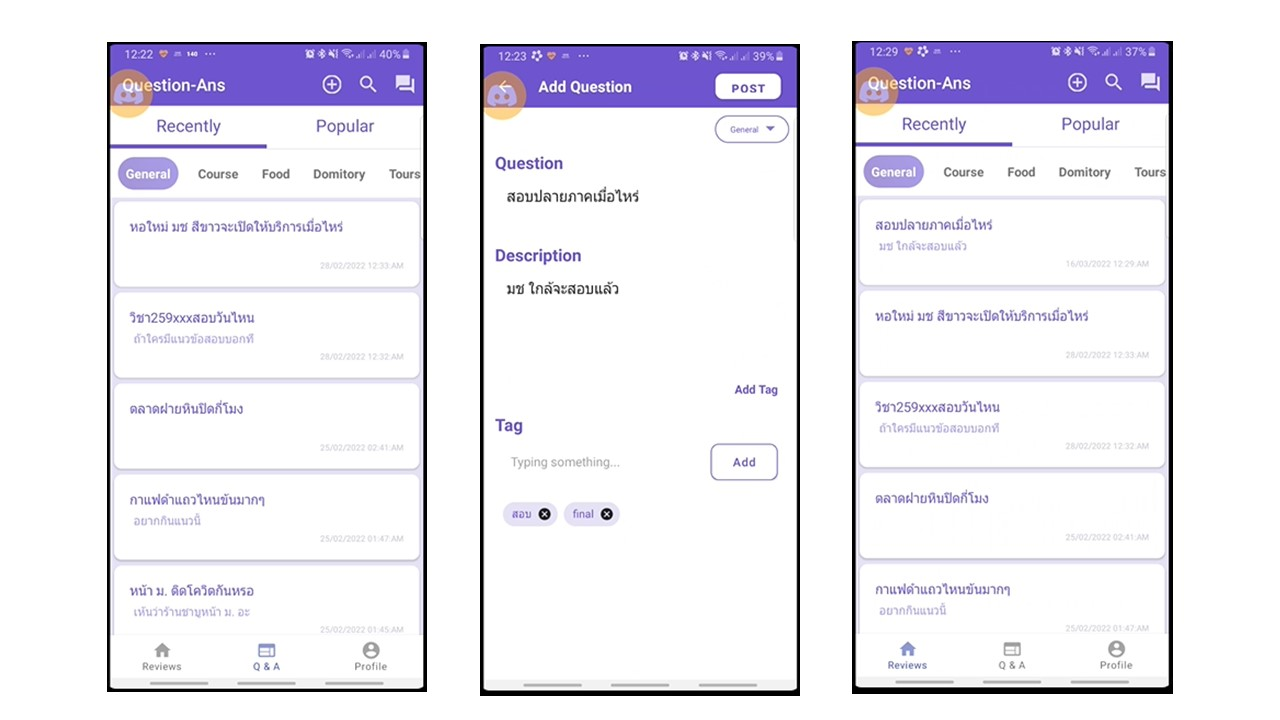
\includegraphics[width=1\textwidth]{./image/testing/Slide9.JPG}
    \end{center}
    \caption[การทดสอบการเพิ่มกระทู้]{การทดสอบการเพิ่มกระทู้}
    \end{figure}

\section{การทดสอบการเพิ่ม usefull comment}
\quad \quad การทดสอบการเพิ่ม usefull comment คือจะเป็นฟังชั่นที่ช่วยแนะนำผู้ที่เข้ามาอ่านกระทู้ได้เข้าใจง่ายๆว่ากระทู้นี้ มีคอมเม้นนี้ที่สามารถช่วยในการแก้ไขปัญหาหรือ
ช่วยแนะนำได้ดี โดยสามารถเพิ่ม usefull comment ได้ก็ต่อเมื่อเป็นเจ้าของกระทู้ เจ้าของกระทู้จะมีเมนูของคอมเม้นปรากฎอยู่เมื่อกดเข้าไปจะแสดงเมนู add usefull comment 
ผลลัพธ์คือสามารถเพิ่ม usefull comment ได้สำเหร็จ ระบบจะมีการแสดงสีของ usefull commentที่ต่างออกไปเพื่อให้มองเห็นได้ง่าย  ดังรูป 4.9

\begin{figure}
    \begin{center}
      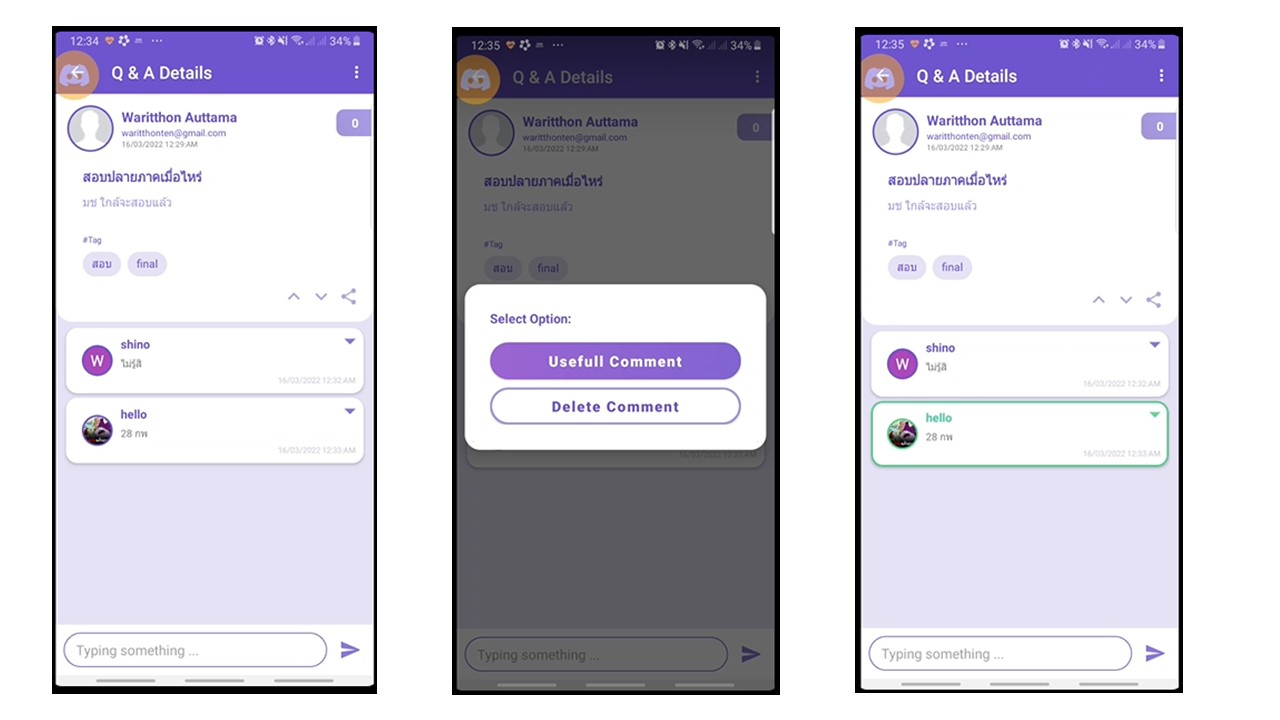
\includegraphics[width=1\textwidth]{./image/testing/Slide10.JPG}
    \end{center}
    \caption[การทดสอบการเพิ่ม usefull comment]{การทดสอบการเพิ่ม usefull comment}
    \end{figure}

\section{การทดสอบการค้นหารีวิว}
\quad \quad การทดสอบการค้นหารีวิว คือฟังชั่นที่สามารถพิมค้นรีวิวหรือกระทู้ก็ได้ โดยการทดลองจะให้พิมค้นหารีวิว hello  
ผลลัพธ์คือระบบจะแสดงรายการที่มีชื่อหรือมีส่วนเกี่ยวข้องกับ hello คำค้นของเรา  ดังรูป 4.10

\begin{figure}
    \begin{center}
      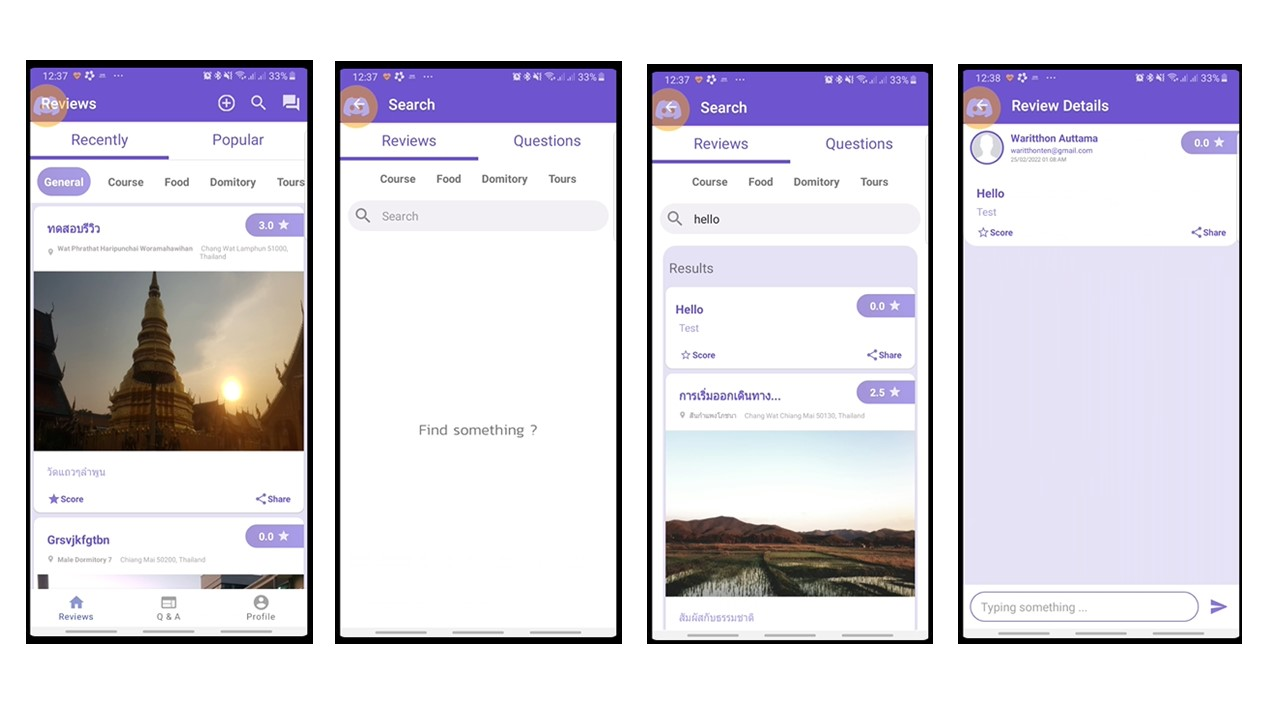
\includegraphics[width=1\textwidth]{./image/testing/Slide11.JPG}
    \end{center}
    \caption[การทดสอบการค้นหารีวิว]{การทดสอบการค้นหารีวิว}
    \end{figure}

\section{การทดสอบการหาเพื่อนและเริ่มการสนทนา}
\quad \quad การทดสอบการหาเพื่อนและเริ่มการสนทนา คือเราสามารถค้นหาเพื่อนที่เราจะเริ่มคุยด้วยได้จากชื่อหรืออีเมล
ผลลัพธ์คือระบบสามารถทำงานค้นหาได้อย่างถูกต้องและสามารถส่งข้อความหาคู่สนทนาได้  ดังรูป 4.11

\begin{figure}
    \begin{center}
      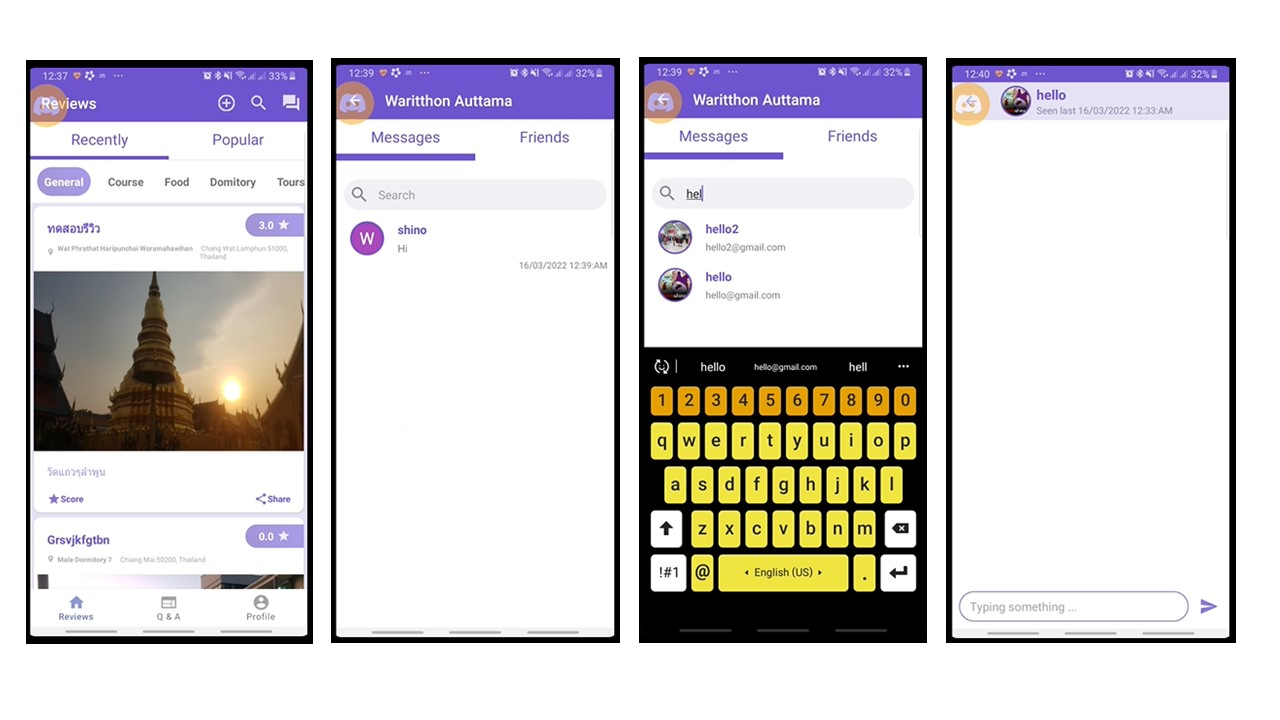
\includegraphics[width=1\textwidth]{./image/testing/Slide12.JPG}
    \end{center}
    \end{figure}

\begin{figure}
    \begin{center}
      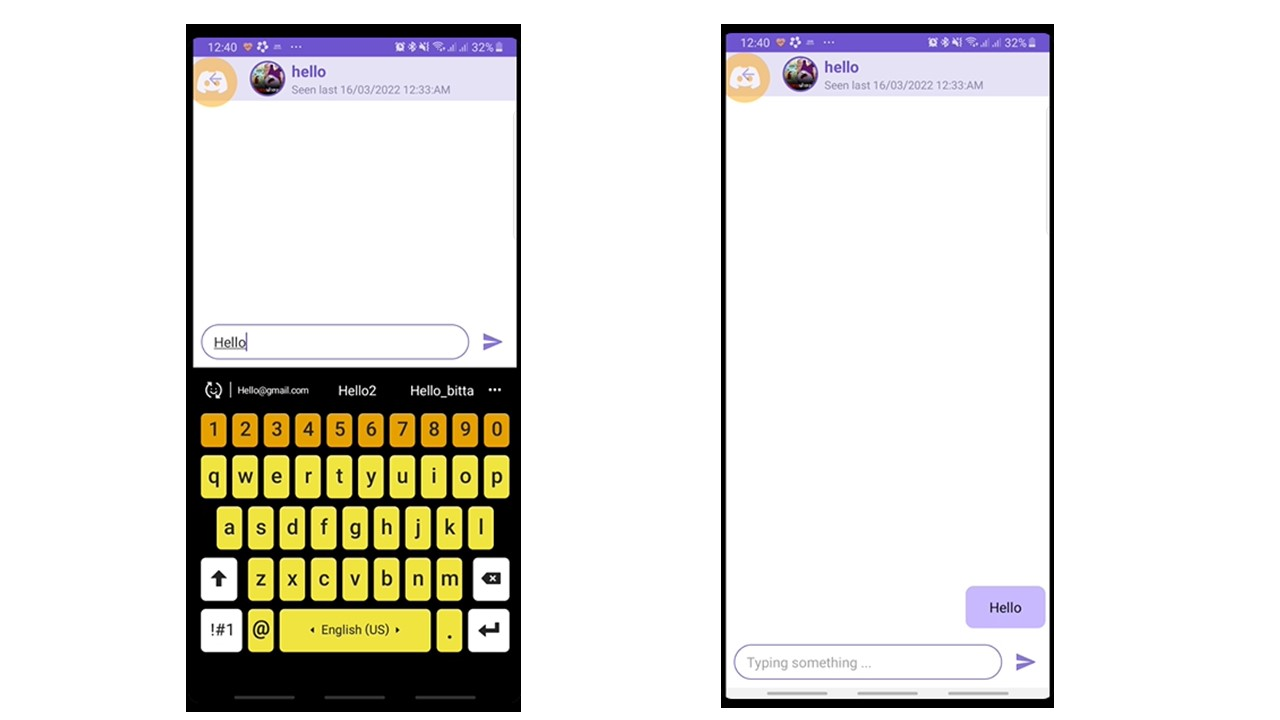
\includegraphics[width=1\textwidth]{./image/testing/Slide13.JPG}
    \end{center}
    \caption[การทดสอบการหาเพื่อนและเริ่มการสนทนา]{การทดสอบการหาเพื่อนและเริ่มการสนทนา}
    \end{figure}